% Enable warnings about problematic code
\RequirePackage[l2tabu, orthodox]{nag}

\documentclass{resources/WeSTassignment}
\usepackage{tabularx}
\usepackage{booktabs}
\usepackage[utf8]{inputenc}
\usepackage{amsmath}
\usepackage{graphics}
\usepackage{graphicx}
\usepackage{changebar}
\usepackage{latexsym}
\usepackage{stmaryrd}
\usepackage{booktabs}
\usepackage{amsmath}
\usepackage{wasysym}
\usepackage[export]{adjustbox}
\usepackage[thinlines]{easytable}
\usepackage{framed}
\usepackage{color}
\usepackage{footnote}
\usepackage{listings}
\usepackage{framed}
\usepackage{tikz}
\usepackage[T1]{fontenc}
\usepackage{lmodern}

% The lecture title, e.g. "Web Information Retrieval".
\lecture{Introduction to Web Science}
% The names of the lecturer and the instructor(s)
\author{%
  PD Dr. Matthias~Thimm\\{\normalsize\mailto{thimm@uni-koblenz.de}} \and
  Ipek~Baris Schlicht\\{\normalsize\mailto{ibaris@uni-koblenz.de}} \and
  Kenneth Skiba\\{\normalsize\mailto{kennethskiba@uni-koblenz.de}}
}
% Assignment number.
\assignmentnumber{4}
% Institute of lecture.
\institute{%
  Institute of Web Science and Technologies\\%
  Department of Computer Science\\%
  University of Koblenz-Landau%
}
% Date until students should submit their solutions.
\datesubmission{08.12.2020, CEST 23:59}
% Date on which the assignments will be discussed in the tutorial.


\begin{document}
\maketitle

\centering \textbf{Team:} Bravo\\
\centering \textbf{Members:}\\
\centering  Gaurav Kumar (220200656)\\
\centering  Pavithree Shetty (220200661)\\
\centering  Nisha Sharma (220202359)\\

\section{XML \hfill{26 Points} \label{xml}}
Consider the following XML document:

\definecolor{javared}{rgb}{0.6,0,0} % for strings
\definecolor{javagreen}{rgb}{0.25,0.5,0.35} % comments
\definecolor{javapurple}{rgb}{0.5,0,0.35} % keywords
\definecolor{javadocblue}{rgb}{0.25,0.35,0.75} % javadoc

\lstset{language=XML,
basicstyle=\ttfamily,
keywordstyle=\color{javapurple}\bfseries,
stringstyle=\color{javared},
commentstyle=\color{javagreen},
morecomment=[s][\color{javadocblue}]{/**}{*/},
numbers=left,
numberstyle=\tiny\color{black},
stepnumber=1,
numbersep=8pt,
tabsize=4,
showspaces=false,
showstringspaces=false
}
\begin{lstlisting}
?xml version="1.1" encoding="UTF-8" ?>
<book>
	<author><publisher>Macmillan</author></publisher>
	<title>Alice Adventures in Wonderland</title>
	<year>1865</year>
</book>
\end{lstlisting}


\subsection{\hfill }
\textbf{Solution:} \\
The above xml document is not valid for the below mentioned reasons: \\
\begin{enumerate}
\item In the declaration line, \textbf{'<'} is missing. The correct way is \\ <?xml version="1.1" encoding="UTF-8" ?>
\item The element tags for author and publisher are not closed in order. The correct order should be \\
<author><publisher>Macmillan</publisher></author>
\end{enumerate} 

\subsection{Well formed XML}
Consider the following information about the best-selling individual books\footnote{Based on \href{https://en.wikipedia.org/wiki/List\_of\_best-selling\_books}{https://en.wikipedia.org/wiki/List\_of\_best-selling\_books}}: 

\begin{table}[h]
\scalebox{0.60}{
\begin{tabular}{|c|c|c|c|c|c|}
\hline
\textbf{Name} & \textbf{Author(s)}     & \textbf{Original language} & \textbf{First published} & \textbf{Approximate sales} & \textbf{Genre} \\ \hline
The Communist Manifesto & Karl Marx and Friedrich Engels & German & 1848  & > 500 million & Political philosophy\\ \hline
A Tale of Two Cities& Charles Dickens & English & 1859  & 200 million & Historical fiction\\ \hline
Harry Potter and the Philopher's Stone & J. K. Rowling& English & 1997  & 120 million & Fantasy, mystery\\ \hline
The Lion, the Witch and the Wardrobe & C.S. Lewis & English & 1950  & 85 million & Fantasy\\ \hline
The Adventures of Pinocchio & Carlo Collodi & Italian & 1881  & > 80 million & Fantasy\\ \hline
\end{tabular}}
\end{table}

Your task is to encode the table above into a well formed XML document. 

\begin{figure}[h]
   			\centering
   			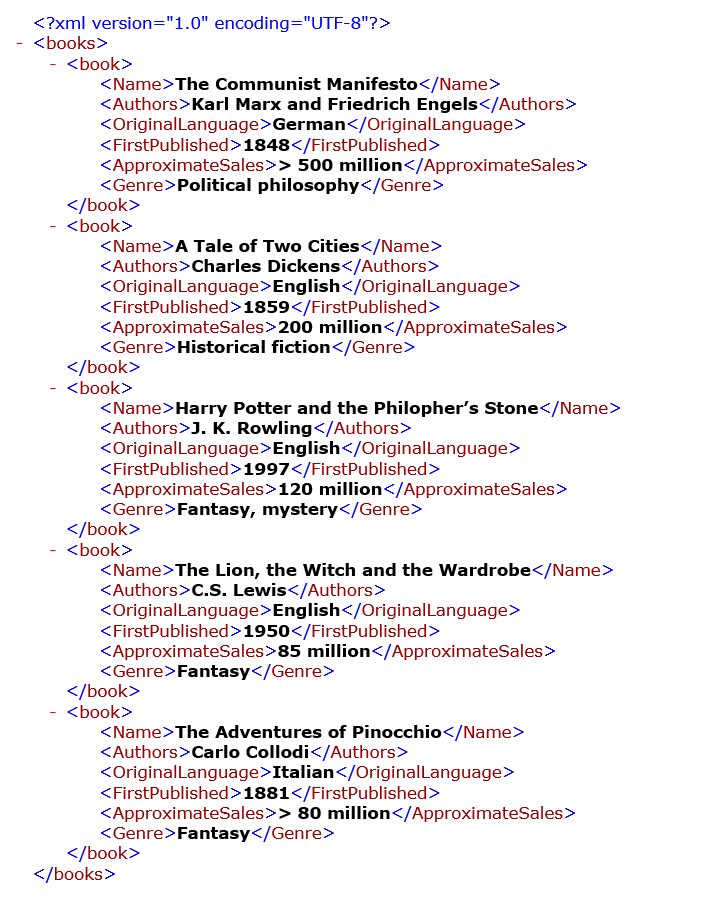
\includegraphics[scale=1.0]{resources/booksXml.PNG}
   			\caption{Output : XML for Above table}
   			\label{fig: BooksXml}
\end{figure}

\section{HTML and CSS\hfill{27 points}\label{html}}
The aim of this task to learn and practice the basics of HTML and CSS. You are required to implement a website that presents your resume. The layout of the website as seen Figure \ref{fig:my_label}. The most left section is \textbf{Experiences}, the middle is the section for \textbf{Education} and the most right section is \textbf{Skills} followed by \textbf{References}.

Perform the following steps:
\begin{enumerate}
    \item Create a HTML file called \texttt{index.html}, and a CSS file called \texttt{style\_display}. In CSS, define the items referring the sections and header and use only \texttt{inline-block} for positioning the items.
    \item Create a CSS file called \texttt{style\_float.css}. In CSS, define the items referring the sections and header and use only \texttt{float} for positioning. Do not alter the contents in \texttt{index.html}.
    \item Create a HTML file called \texttt{index\_table.html}, and a CSS file called \texttt{style\_table.css}. This time, you are supposed to implement the layout by using tables in HTML. However, for styling the cells and the properties of the table, you need to edit the \texttt{style\_table.css}.
\end{enumerate}

Three steps that you will implement should output same layout and content. However, small margins between the results could be neglected. The background color of the sections is \texttt{\#ccc}.

For this task, \textcolor{red}{don't use frameworks such as bootstrap.} You are only allowed to use standard HTML and CSS items. 

\begin{figure}[h]
   	\centering
   	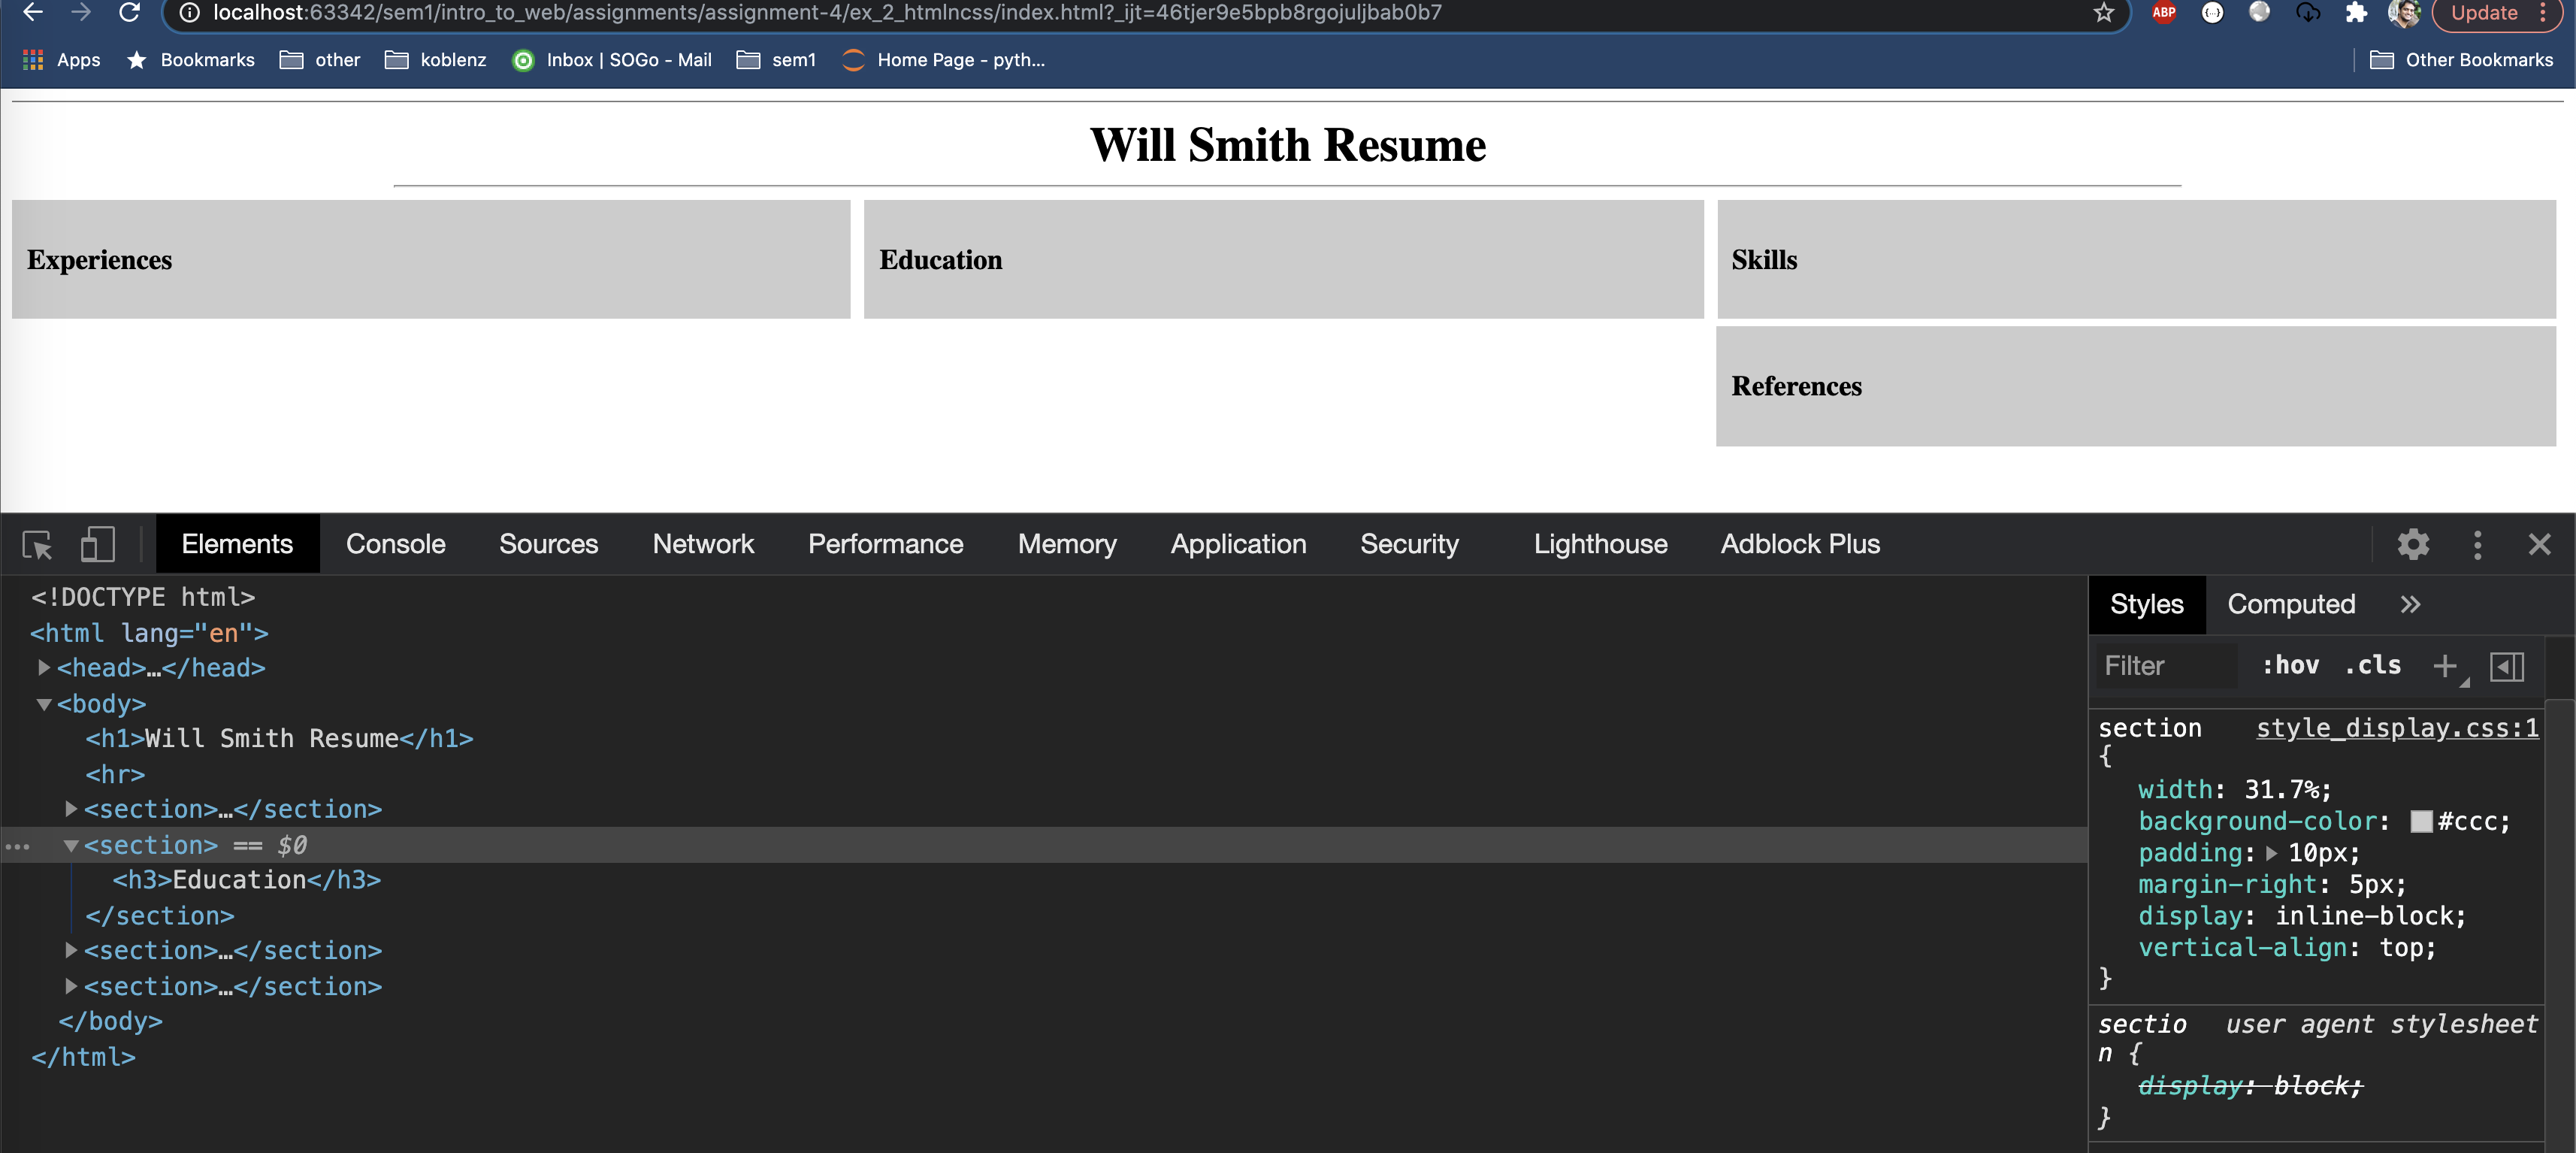
\includegraphics[scale=1.0,width=\linewidth]{html_css/inline-block.png}
   	\caption{With using inline-block style}
   	\label{fig: With using inline-block style}
\end{figure}

\begin{figure}[h]
   	\centering
   	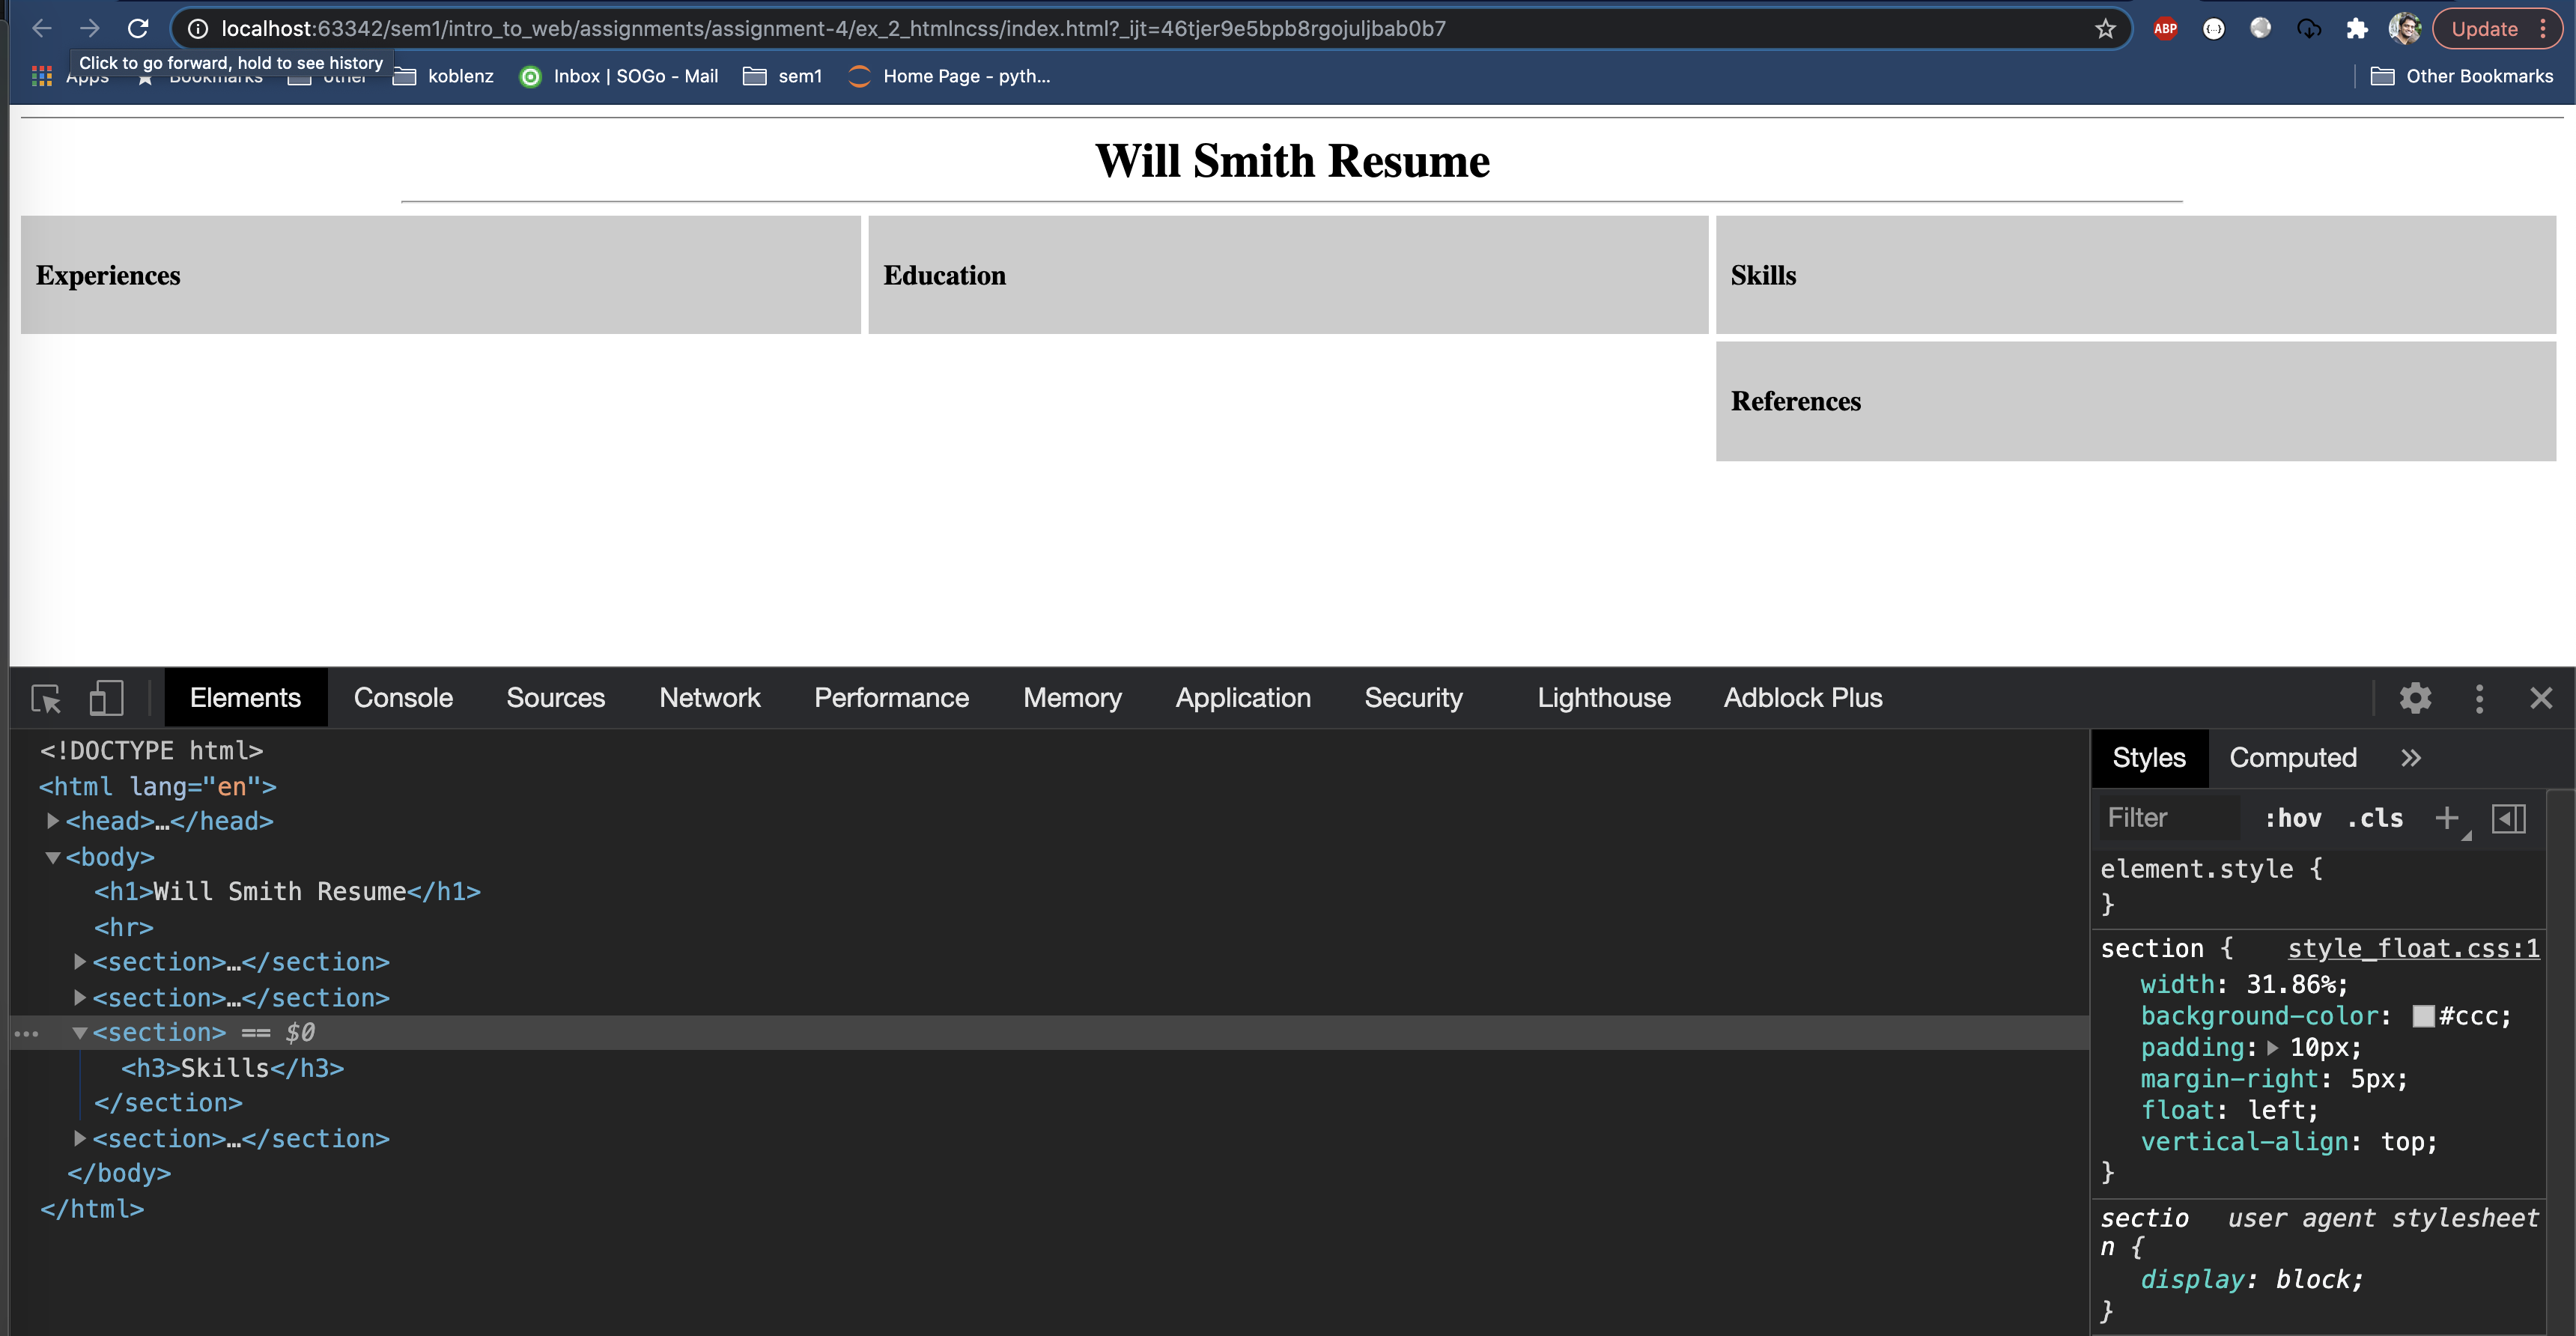
\includegraphics[scale=1.0,width=\linewidth]{html_css/float.png}
   	\caption{With using float style}
   	\label{fig: With using float style}
\end{figure}

\begin{figure}[h]
   		\centering
   		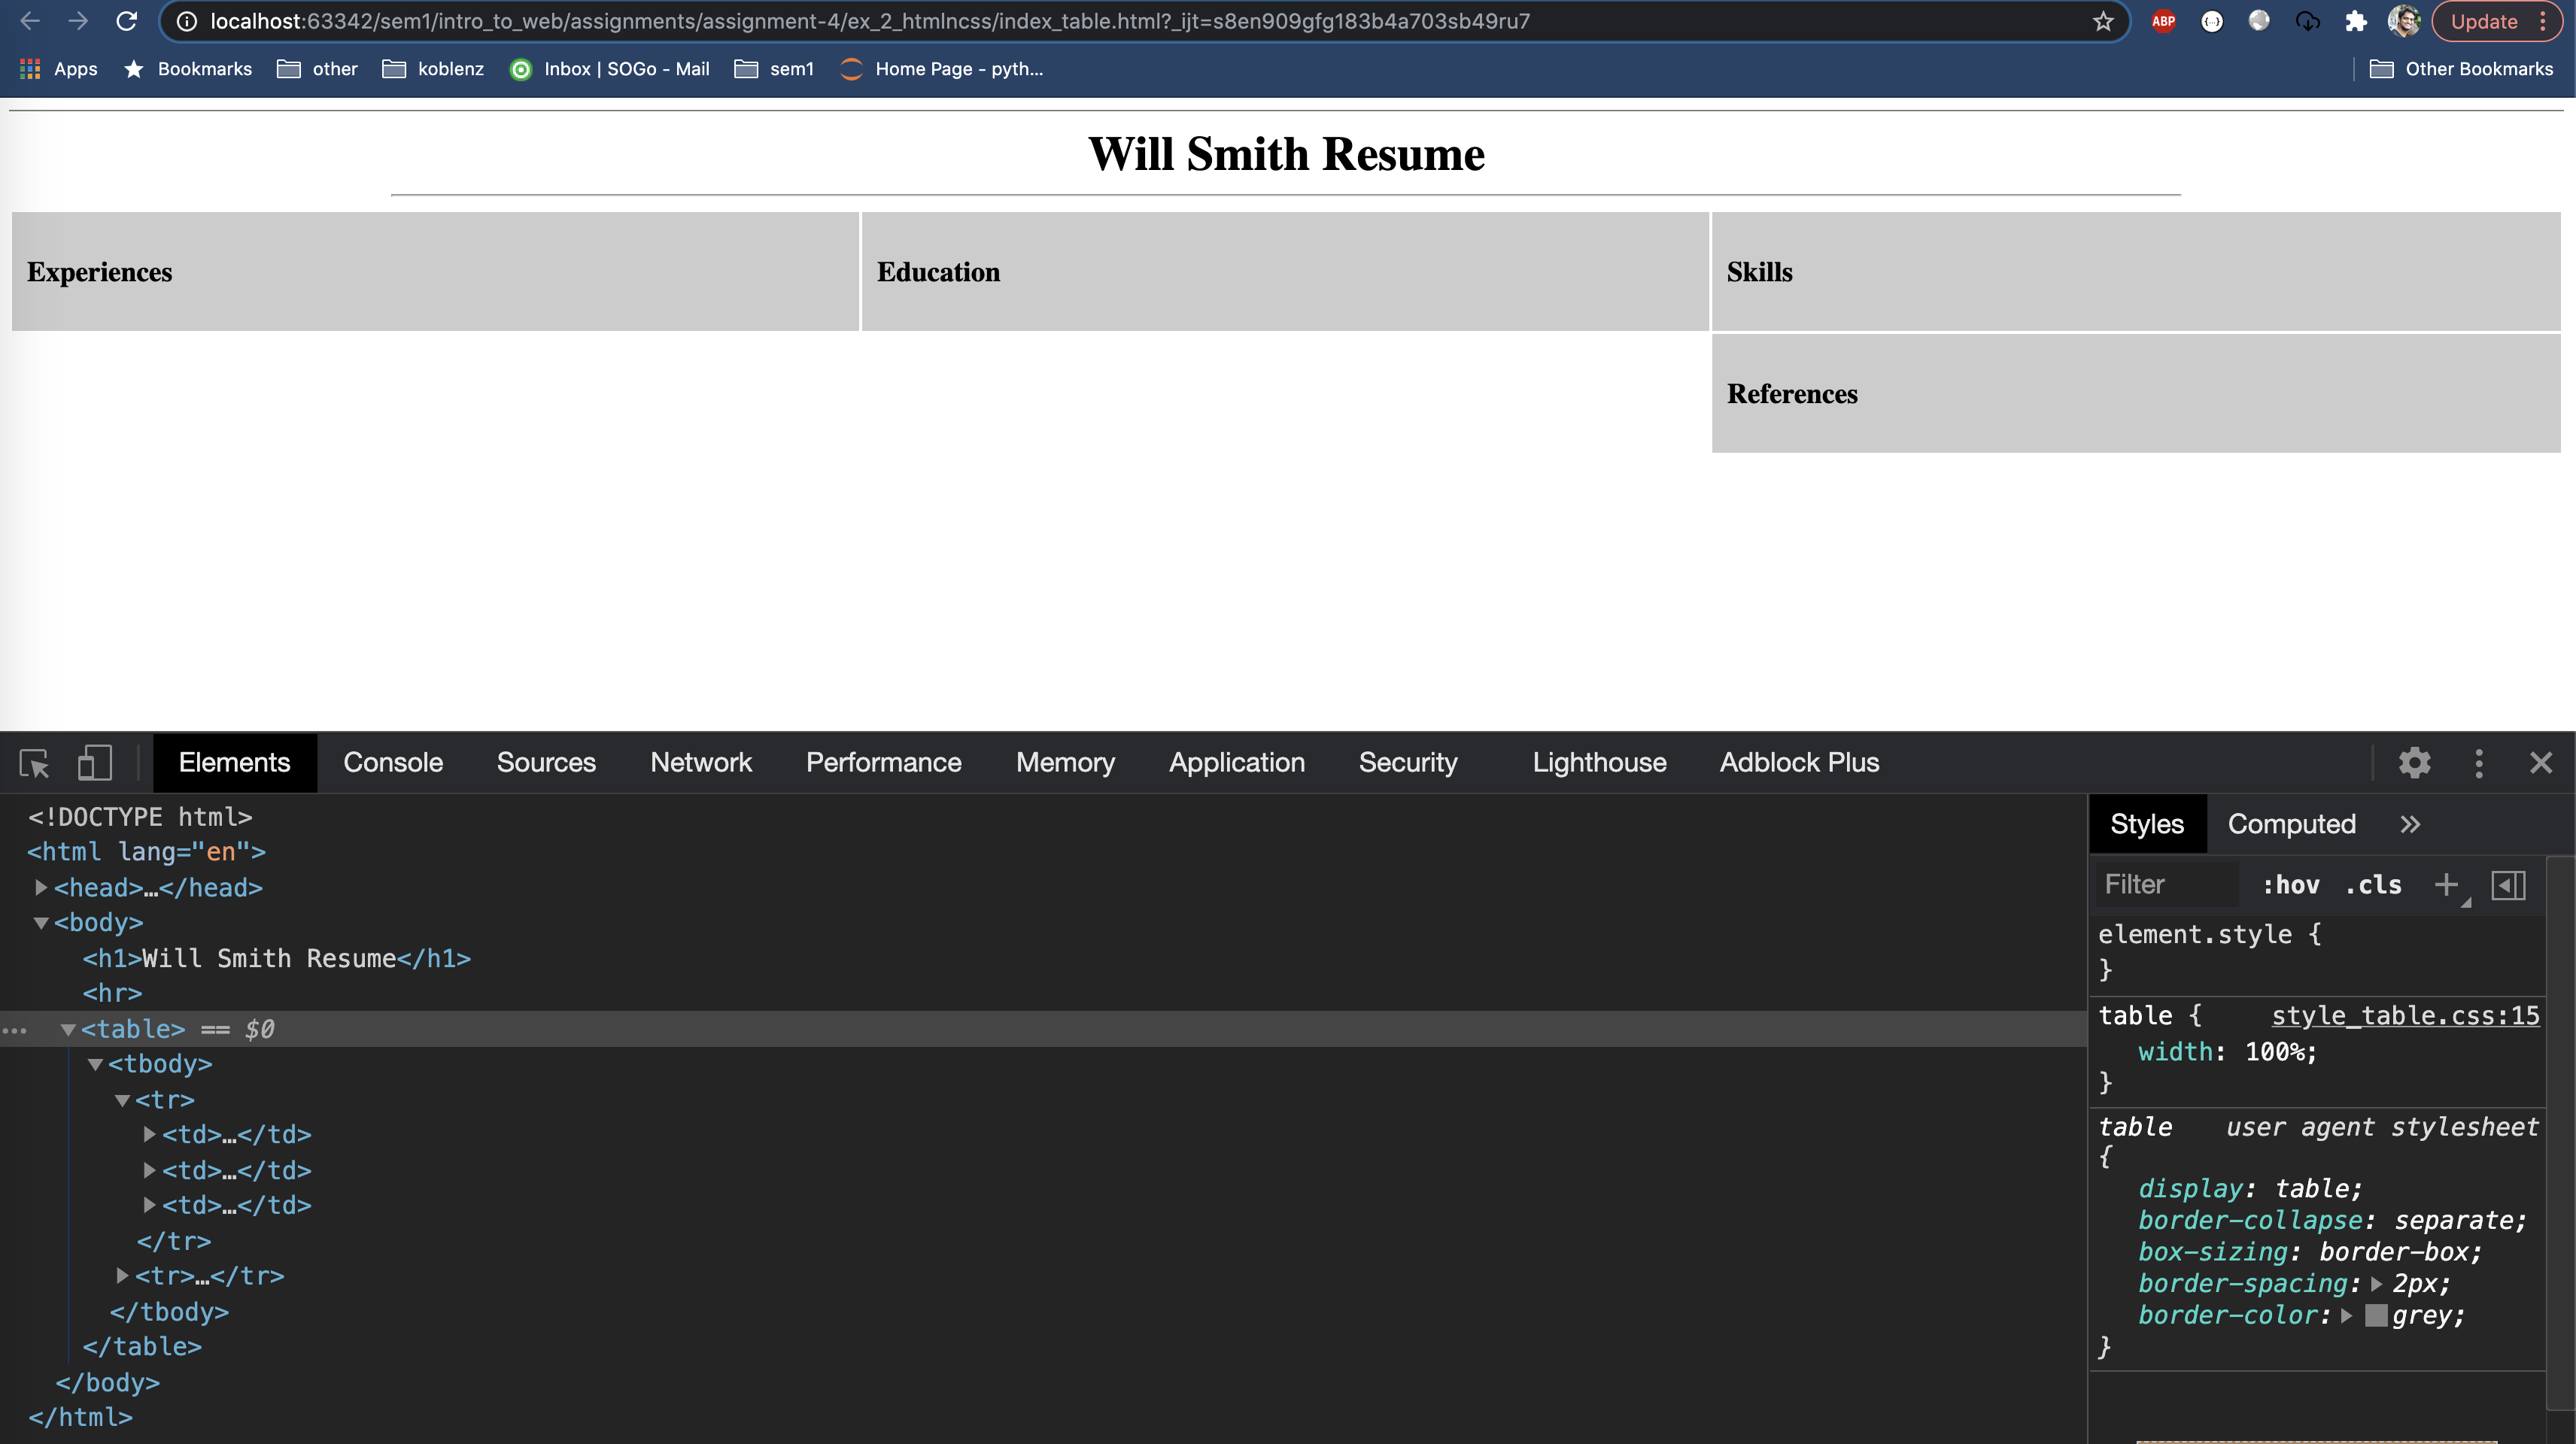
\includegraphics[scale=1.0,width=\linewidth]{html_css/table.png}
   		\caption{With using table template}
   		\label{fig: With using table template}
	\end{figure}

\section{Dynamic Web Content \hfill{27 points}}

	   \begin{figure}[ht]
    			\centering
    			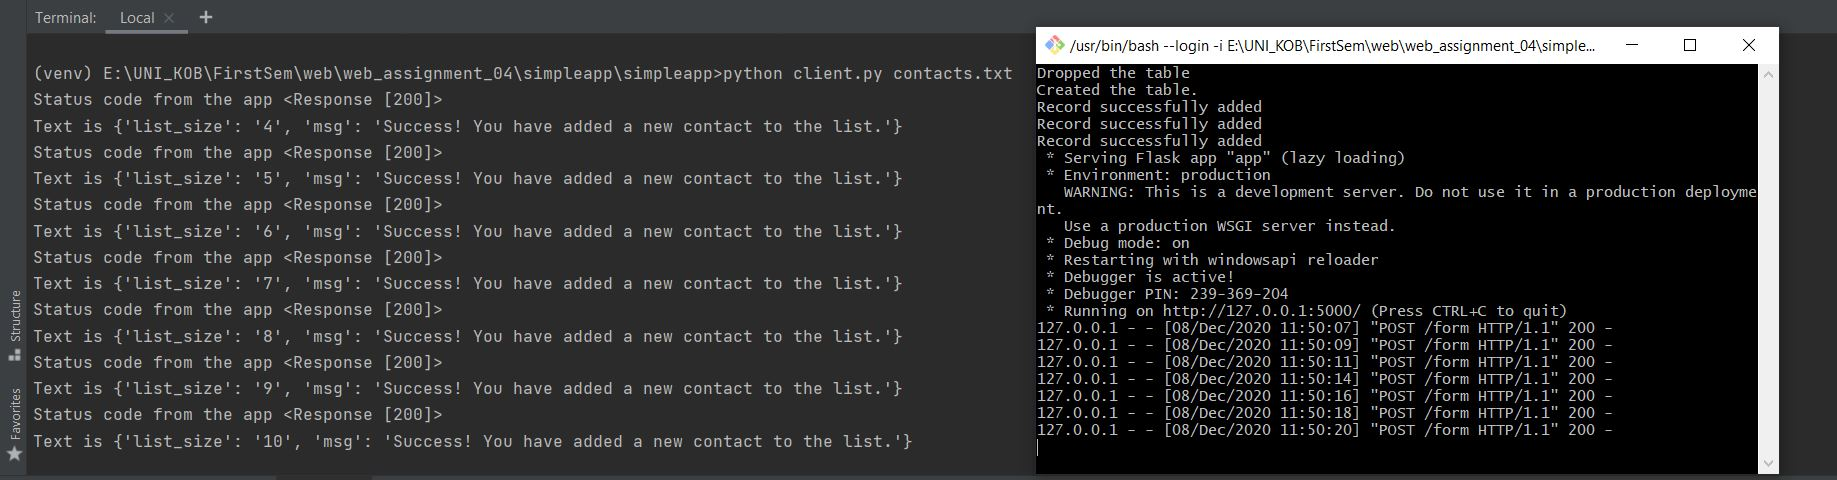
\includegraphics[scale=0.4]{resources/finalContactsServer.JPG}
    			\caption{Output : Contacts.txt}
    			\label{fig:contacts.txt}
\end{figure}

		\begin{figure}[ht]
    			\centering
    			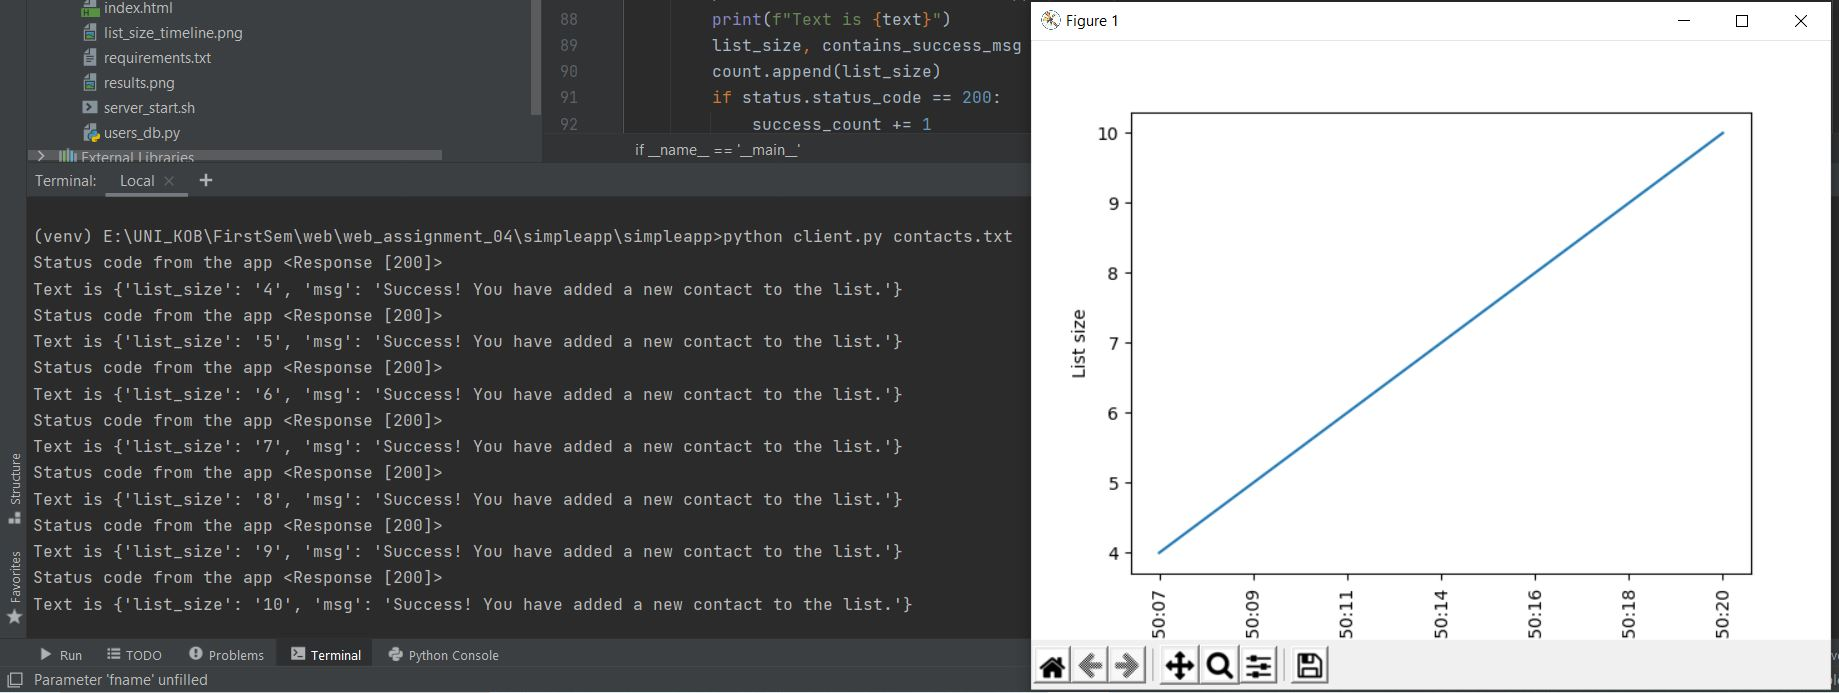
\includegraphics[scale=0.4]{resources/finalContactstimeline.JPG}
    			\caption{Output : Timeline Plot-Contacts.txt}
    			\label{fig:Timeline Plot Contacts.txt}
\end{figure}

		\begin{figure}[ht]
    			\centering
    			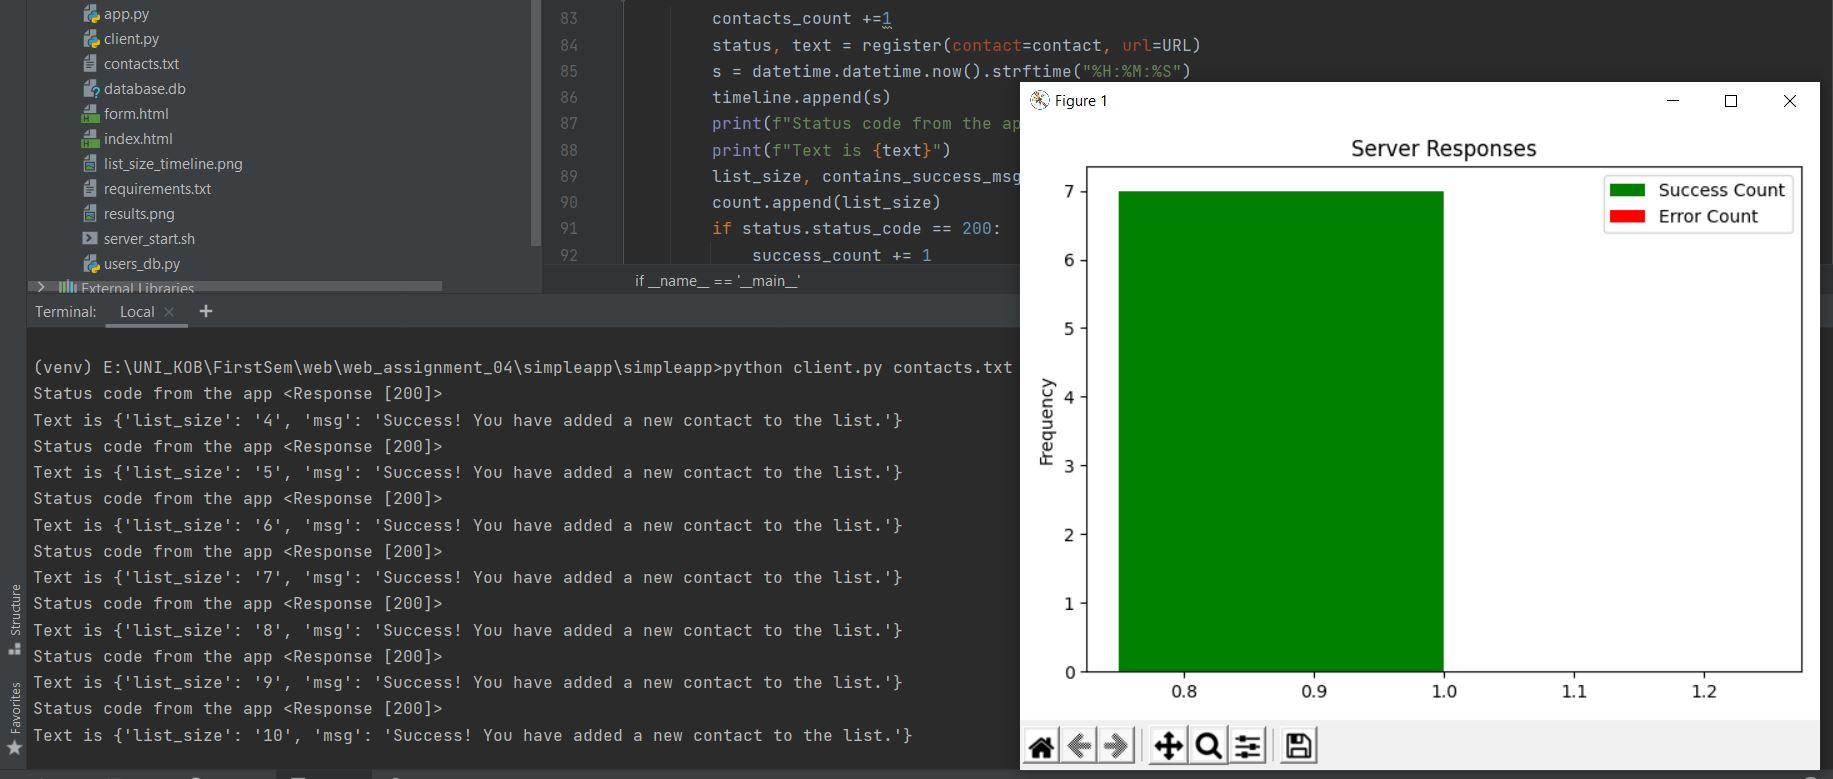
\includegraphics[scale=0.4]{resources/finalContactBarPlot.JPG}
    			\caption{Output : Bar Plot-Contact.txt}
    			\label{fig: BarPlot - Contacts.txt}
\end{figure}

		\begin{figure}[ht]
    			\centering
    			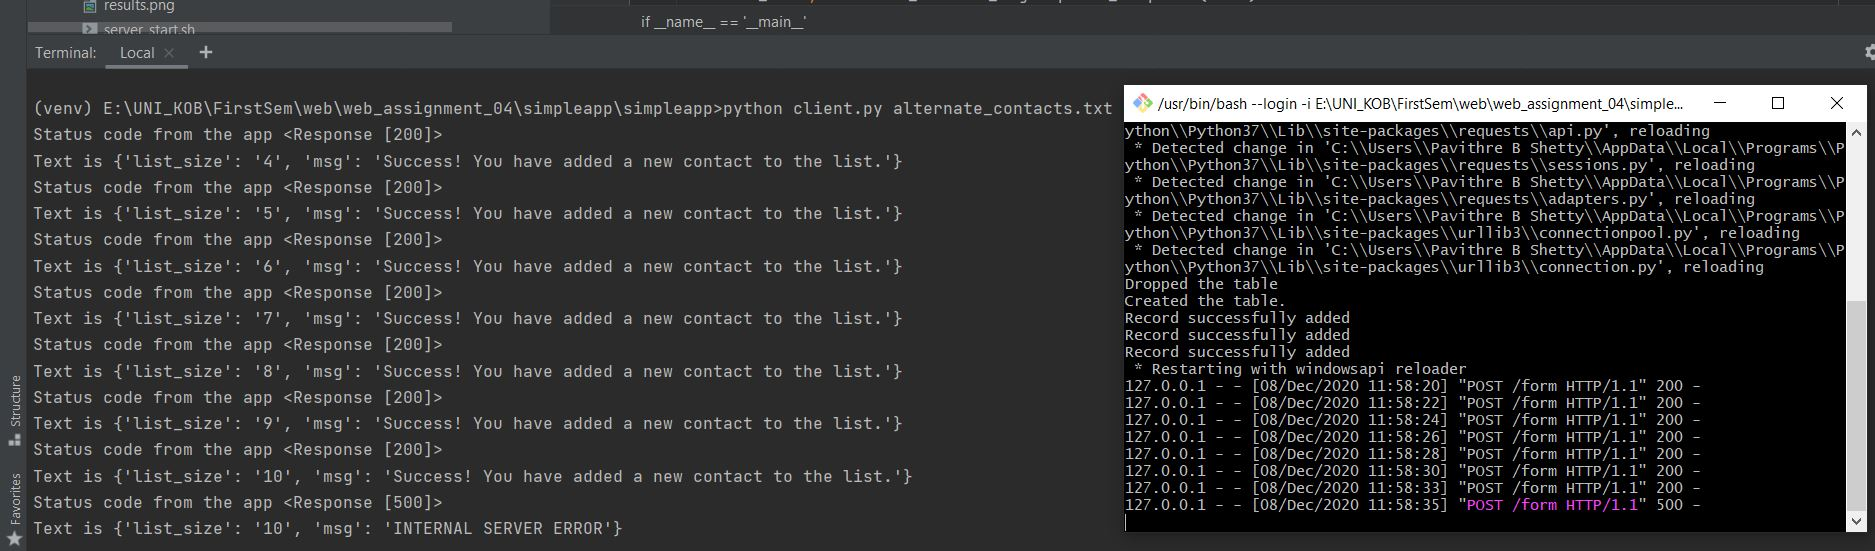
\includegraphics[scale=0.4]{resources/finalAlternateServer.JPG}
    			\caption{Output : AlternateContacts.txt}
    			\label{fig: AlternateContacts.txt}
\end{figure}
 \begin{figure}[ht]
   			\centering
   			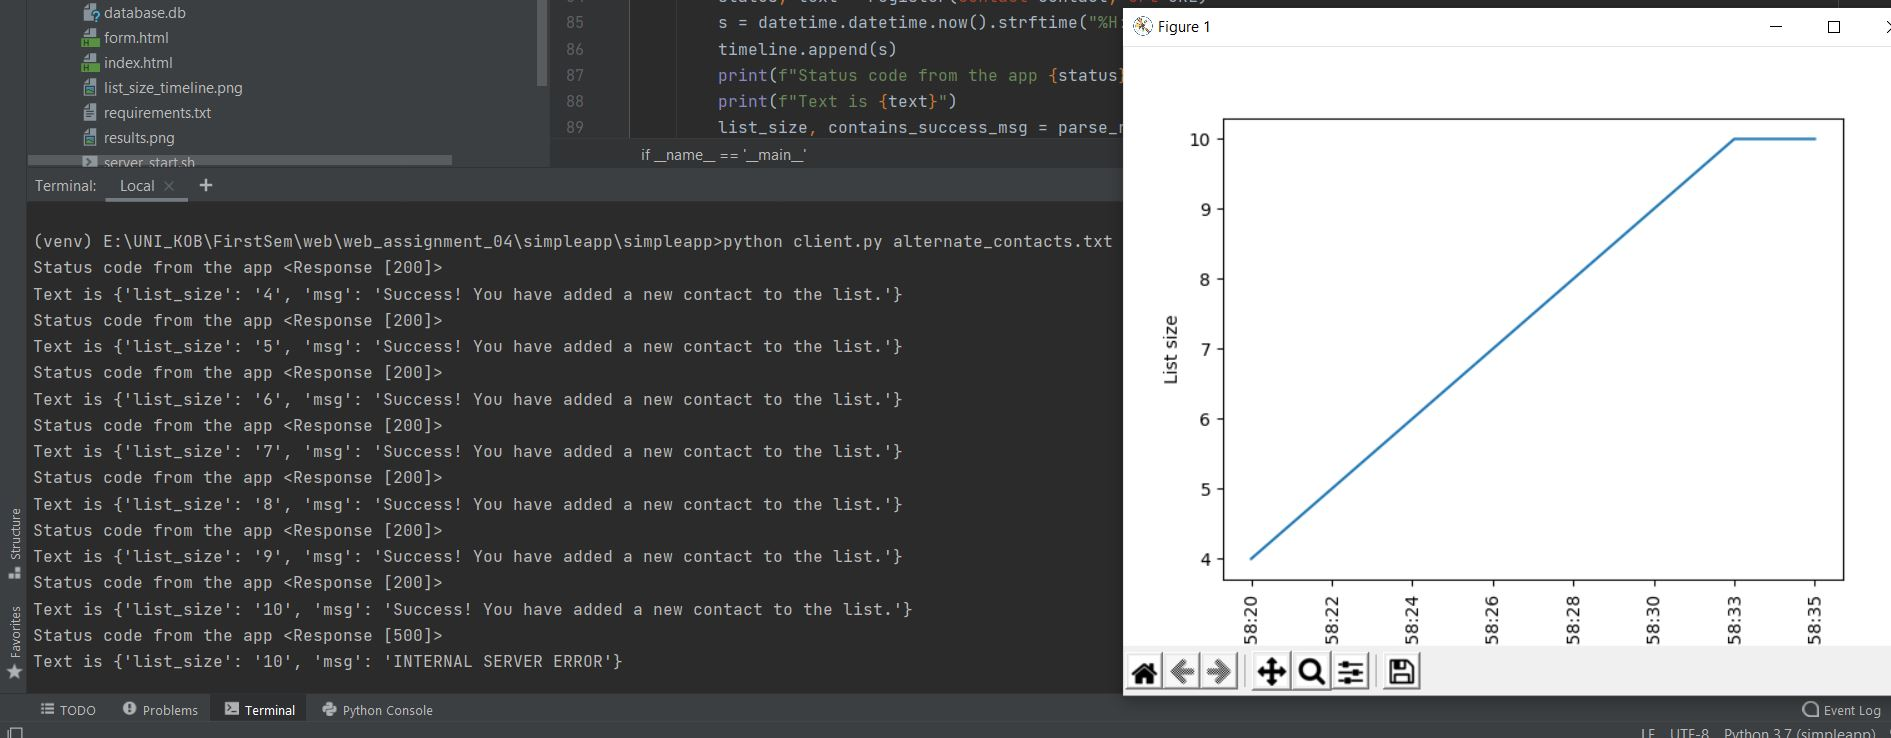
\includegraphics[scale=0.4]{resources/finalAlternateTimeline.JPG}
   			\caption{Output : Timeline Plot AlternateContacts.txt}
   			\label{fig: Timeline Plot - AlternateContacts.txt}
\end{figure}
 \begin{figure}[ht]
   			\centering
   			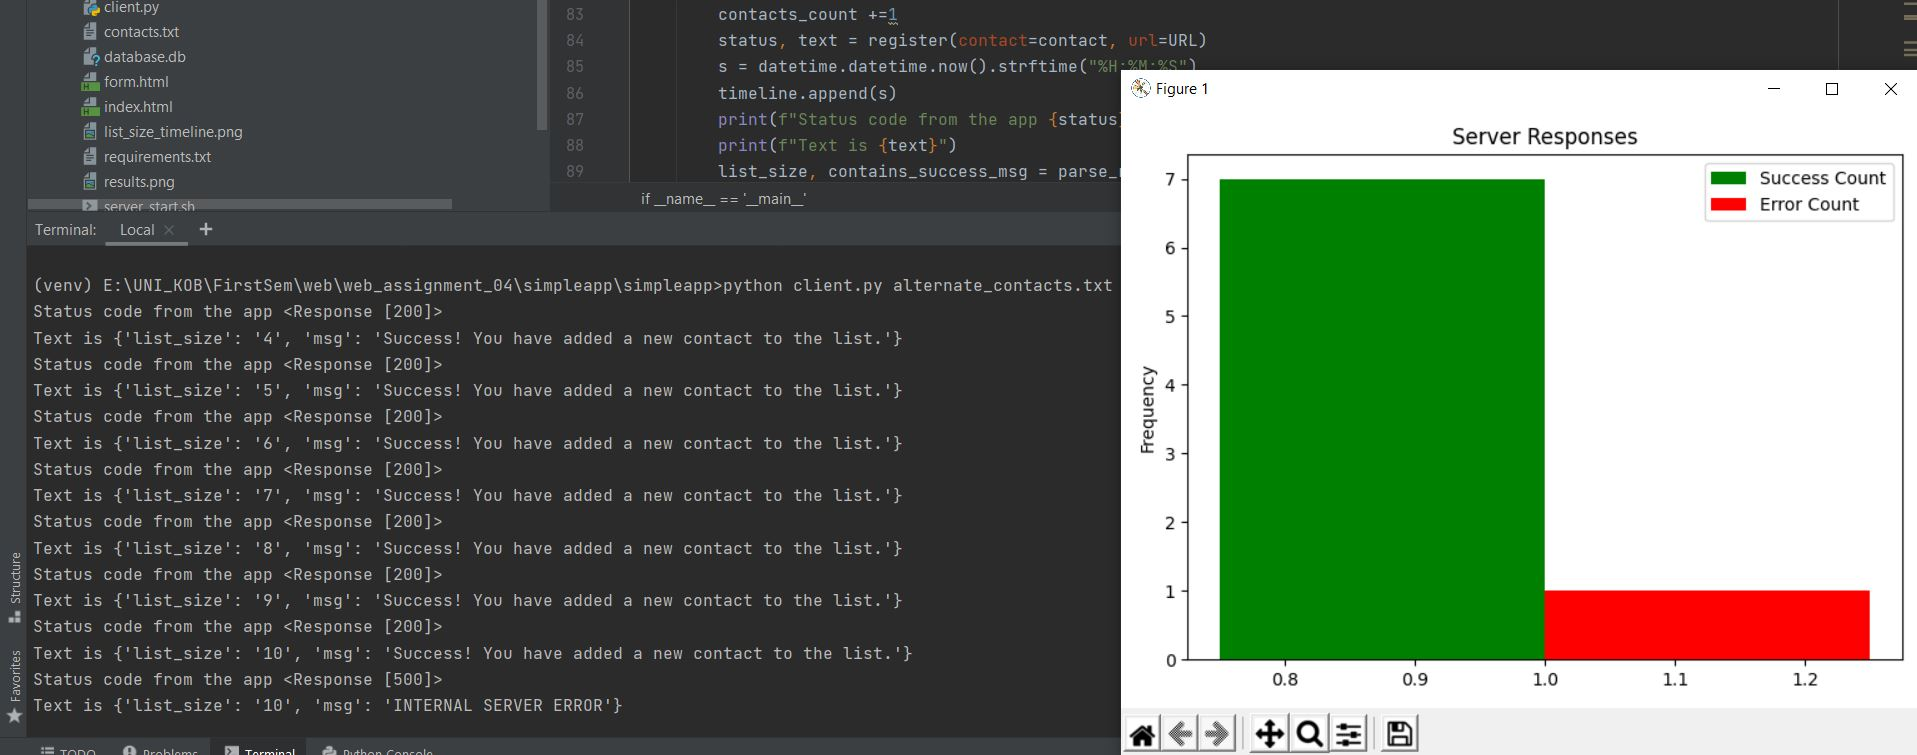
\includegraphics[scale=0.4]{resources/finalAlternateBarPlot.JPG}
   			\caption{Output : Bar Plot - AlternateContacts.txt}
   			\label{fig: Bar Plot-AlternateContacts.txt}
\end{figure}
\begin{figure}[ht]
   			\centering
   			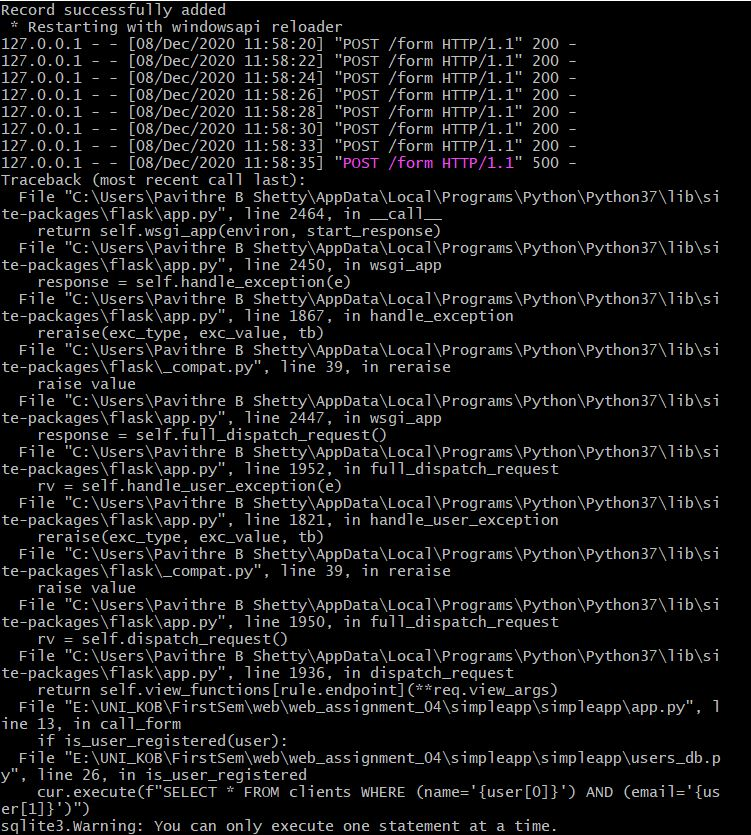
\includegraphics[scale=0.4]{resources/finalAlternateServerError.JPG}
   			\caption{Output : Server Error AlternateContacts.txt}
   			\label{fig: Server Error AlternateContacts.txt}
\end{figure}
\begin{enumerate}
\item The execute() for the query "SELECT * FROM clients WHERE (name='{user[0]}') AND (email='{user[1]}')" in user.db can execute only a single execute statement. 
\item The input "Ipek, dummy@gmail.com'); DROP TABLE clients; --; INSERT INTO clients VALUES (Kenneth, dummy2@mail.com" has multiple lines which cannot be executed with excecute() for the above query. Thats why we get the warning as "You can execute only one statement at a time"
\end{enumerate}





\end{document}
